\documentclass[a4paper,11pt]{article}

\usepackage[utf8]{inputenc}
\usepackage[T1]{fontenc}
\usepackage{lmodern}
\usepackage[english]{babel}
\usepackage{microtype}
\usepackage{geometry}
\usepackage{graphicx}
\usepackage{booktabs}
\usepackage{tabularx}
\usepackage{longtable}
\usepackage{float}
\usepackage{xcolor}
\usepackage{hyperref}
\usepackage{siunitx}
\usepackage[backend=biber,style=numeric,sorting=none]{biblatex}

\geometry{left=25mm,right=25mm,top=25mm,bottom=28mm}
\hypersetup{
  colorlinks=true,
  linkcolor=black,
  citecolor=black,
  urlcolor=blue
}
\sisetup{
  round-mode=places,
  round-precision=4
}
\addbibresource{references.bib}

\newcommand{\todo}[1]{\textcolor{red}{\textbf{TODO:} #1}}
\newcommand{\runpath}{\texttt{outputs/experiments/course\_practical}}

\title{Land Use Classification on EuroSAT}
\author{
  Andreas Glashauser \\
  Patrick Hübler \\
  Tobias Litke \\
  Deep Learning and Big Data
}
\date{\today}

\begin{document}

\maketitle

\tableofcontents
\newpage

\section{Introduction}

Satellite images contain useful information about land use and land cover. This
makes automatic classification of such images a natural application for deep
learning. In this project, the EuroSAT RGB dataset is used
\cite{helber2019eurosat,eurosatgithub}.

The project compares two model approaches on the same dataset. Model 1 is a CNN
trained from scratch. Its purpose is to show the full training process, from
architecture design to optimizer choice and evaluation. Model 2 is a transfer
learning approach, in which an ImageNet-pretrained convolutional backbone is
fine-tuned on EuroSAT. To avoid drawing conclusions from a single architecture,
the transfer learning approach is evaluated with two structurally different
backbones: the parameter-efficient EfficientNet-B0
\cite{tan2019efficientnet,pytorch} and the larger deep-residual ResNet-50
\cite{he2016resnet}. Comparing two backbones shows whether any advantage over
the scratch CNN comes from transfer learning in general rather than from one
specific model, and lets us study how pretrained features affect accuracy and
data efficiency across architectures.

Two tasks are considered on the same dataset:

\begin{itemize}
  \item a 10-class classification task using the original EuroSAT classes,
  \item a binary classification task: vegetation vs. non-vegetation.
\end{itemize}

The same train/validation/test split was used for both tasks. This is important
because otherwise differences in the results could also come from different
data partitions. The hyperparameter experiments used only the training and
validation splits. The test split was evaluated only for the final selected
configurations.

\section{Dataset and Tasks}

\subsection{EuroSAT RGB}

The dataset used in this project is EuroSAT RGB. It contains 27\,000 RGB images
with a resolution of 64 x 64 pixels. Each image belongs to exactly one of ten
land-use classes. Since the RGB version was used, only the red, green, and blue
channels were available. Additional Sentinel-2 spectral bands were not used in
this project.

\begin{table}[H]
\centering
\caption{Class distribution and split used in this project.}
\label{tab:split}
\begin{tabular}{lrrrr}
\toprule
Class & Total & Train & Validation & Test \\
\midrule
AnnualCrop & 3000 & 2100 & 450 & 450 \\
Forest & 3000 & 2100 & 450 & 450 \\
HerbaceousVegetation & 3000 & 2099 & 451 & 450 \\
Highway & 2500 & 1750 & 375 & 375 \\
Industrial & 2500 & 1750 & 375 & 375 \\
Pasture & 2000 & 1400 & 300 & 300 \\
PermanentCrop & 2500 & 1750 & 375 & 375 \\
Residential & 3000 & 2100 & 450 & 450 \\
River & 2500 & 1750 & 375 & 375 \\
SeaLake & 3000 & 2100 & 450 & 450 \\
\midrule
\textbf{Total} & \textbf{27000} & \textbf{18899} & \textbf{4051} & \textbf{4050} \\
\bottomrule
\end{tabular}
\end{table}

The split was created in a stratified way with seed 42. This keeps the class
distribution in the training, validation, and test splits as similar as
possible. The small differences are caused by rounding for classes with 2500 or
3000 images.

\subsection{Binary Task}

In addition to the original 10-class task, a binary task was defined. The
classes were grouped into vegetation and non-vegetation:

\begin{table}[H]
\centering
\caption{Mapping used for binary classification.}
\label{tab:binary_mapping}
\begin{tabularx}{\textwidth}{lX}
\toprule
Binary class & EuroSAT classes \\
\midrule
Vegetation & AnnualCrop, Forest, HerbaceousVegetation, Pasture, PermanentCrop \\
Non-vegetation & Highway, Industrial, Residential, River, SeaLake \\
\bottomrule
\end{tabularx}
\end{table}

This second task is useful because it uses the same dataset but asks a different
question. It is also less fine-grained than the 10-class task. Therefore, it is
expected to be easier, because several visually similar vegetation classes are
merged into one class.

\subsection{Preprocessing}

To avoid data leakage, the split was created before any normalization
statistics were computed. The mean and standard deviation were then computed
only on the training split. The RGB statistics used were:

\begin{itemize}
  \item Mean: [0.3448, 0.3806, 0.4083]
  \item Standard deviation: [0.2031, 0.1371, 0.1156]
\end{itemize}

Training images were optionally augmented. In the final configuration this
included horizontal flips, vertical flips, and rotations up to 15 degrees. No
random augmentation was applied to validation or test images. Those images were
only converted to tensors and normalized with the training statistics.

\begin{figure}[H]
\centering
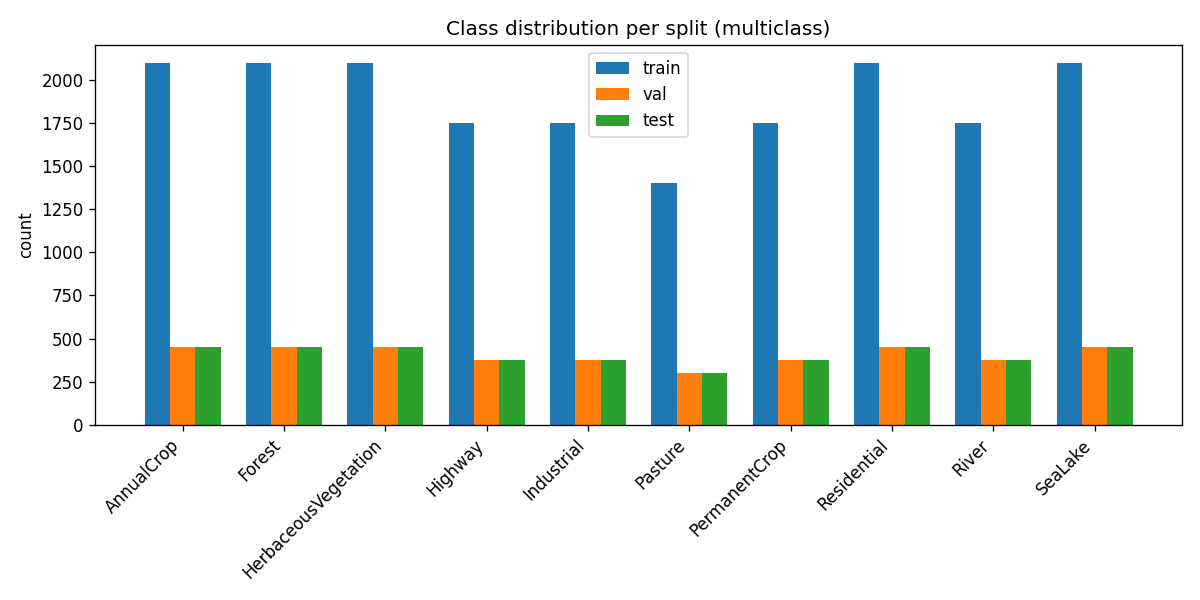
\includegraphics[width=0.85\textwidth]{../outputs/experiments/course_practical/runs/Final_multiclass/plots/class_distribution.png}
\caption{Class distribution in the final 10-class experiment.}
\label{fig:class_distribution}
\end{figure}

\section{Model 1: Scratch CNN}
\label{sec:model1}

\subsection{Methods}

The first model is a small Convolutional Neural Network trained from scratch.
It was kept compact on purpose, because the input images are only 64 x 64
pixels and the model is trained without pretrained weights. The architecture
consists of four convolution blocks and one linear classifier.

\begin{table}[H]
\centering
\caption{Architecture of the scratch CNN.}
\label{tab:architecture}
\begin{tabularx}{\textwidth}{lXX}
\toprule
Stage & Layers & Output idea \\
\midrule
Input & RGB image & 3 x 64 x 64 \\
Block 1 & Conv2d 3->32, ReLU, MaxPool & 32 x 32 x 32 \\
Block 2 & Conv2d 32->64, ReLU, MaxPool & 64 x 16 x 16 \\
Block 3 & Conv2d 64->128, ReLU, MaxPool & 128 x 8 x 8 \\
Block 4 & Conv2d 128->256, ReLU, AdaptiveAvgPool & 256 x 1 x 1 \\
Classifier & Flatten, Dropout, Linear & 10 or 2 logits \\
\bottomrule
\end{tabularx}
\end{table}

A CNN was chosen because the images contain local spatial patterns.
Convolutional layers can learn local structures such as vegetation areas,
roads, water surfaces, or dense buildings. ReLU was used as the activation
function because it adds nonlinearity and is simple and stable in deep
networks.

Max pooling reduces the spatial resolution after the first three blocks. This
lowers the computational cost and forces the model to learn more abstract
features. The last block uses adaptive average pooling to 1 x 1, which keeps
the number of parameters before the classifier small.

The model outputs raw logits. No Softmax layer is included in the model during
training. Instead, \texttt{CrossEntropyLoss} is used, which in PyTorch works
directly with logits \cite{pytorch}.

The training loop follows the procedure used in the course: compute
predictions, compute the loss, calculate gradients with backpropagation,
perform the optimizer step, and reset the gradients. The checkpoint with the
lowest validation loss was saved.

The final configuration was selected from the validation experiments in
Section \ref{sec:model1_experiments}. It uses:

\begin{itemize}
  \item \texttt{CrossEntropyLoss},
  \item SGD with momentum 0.9,
  \item learning rate 0.01,
  \item weight decay 1e-4,
  \item dropout 0.3,
  \item batch size 64,
  \item up to 50 epochs.
\end{itemize}

For the 10-class task, the final linear layer has ten outputs. For the binary
task, the same architecture is used with two outputs. This keeps both tasks
directly comparable.

\subsection{Experimental Design}
\label{sec:model1_experiments}

Several experiments were run on the 10-class task to select the final scratch
CNN configuration. The binary task was trained only after this selection. This
keeps the scratch-CNN model selection focused on the harder task.

The ablations E1 to E5 are evaluated only on training and validation data. The
test split was not used for these decisions, because the test split should
remain an independent estimate of the final model performance.

\begin{table}[H]
\centering
\caption{Experiment campaign for the scratch CNN. Test metrics were deliberately
not computed for ablation runs.}
\label{tab:experiments}
\small
\begin{tabularx}{\textwidth}{lXlrrrr}
\toprule
ID & Purpose & Opt. & Epochs & Val Loss & Val Acc. & Val F1 \\
\midrule
E0 & overfit sanity check on 100 images & Adam & 50 & 0.6806 & 0.7400 & 0.7395 \\
E1 & baseline without augmentation & Adam & 29 & 0.1618 & 0.9437 & 0.9419 \\
E2 & augmentation & Adam & 35 & 0.1639 & 0.9472 & 0.9456 \\
E3 & augmentation + dropout/L2 & Adam & 47 & 0.1522 & 0.9504 & 0.9489 \\
E4 & same as E3, but SGD+momentum & SGD & 50 & 0.1362 & 0.9573 & 0.9557 \\
E5 & depthwise-separable convolutions & SGD & 50 & 0.2568 & 0.9121 & 0.9104 \\
\bottomrule
\end{tabularx}
\end{table}

E0 was intended as a sanity check. The model learned the small 100-image subset
clearly better than random guessing, but it did not fully memorize it. The
maximum training accuracy was 0.75. Therefore, E0 should not be interpreted as
a perfect overfitting result, but as evidence that the training loop, model,
and labels are working.

The comparison between E1 and E2 shows a small benefit from augmentation. The
macro-F1 increased from 0.9419 to 0.9456. The validation loss became slightly
worse. For model selection, macro-F1 was more important because it summarizes
performance across all classes and not only the average confidence of the
model.

E3 adds dropout and L2 regularization. This improved the macro-F1 to 0.9489 and
reduced the validation loss to 0.1522. This supports the use of
regularization.

The best validation result was achieved by E4. Compared with E3, only the
optimizer was changed: Adam was replaced by SGD with momentum 0.9. This raised
the macro-F1 to 0.9557 and reduced the validation loss to 0.1362. Therefore,
this configuration was selected for the final runs.

E5 tested whether replacing the standard convolutions with depthwise-separable
convolutions could reduce the model size while keeping similar validation
performance. This variant used 48,424 trainable parameters instead of 390,986.
However, the validation macro-F1 dropped from 0.9557 in E4 to 0.9104 in E5.
The parameter reduction therefore came with a substantial performance cost, so
E5 was not selected for the final test evaluation.

\subsection{Results}

\subsubsection{Final 10-Class Classification}

The final 10-class classification uses the configuration selected in E4. Table
\ref{tab:final_multiclass} shows the validation and test results.

\begin{table}[H]
\centering
\caption{Final results for the 10-class classification task.}
\label{tab:final_multiclass}
\begin{tabular}{lrr}
\toprule
Metric & Validation & Test \\
\midrule
Loss & 0.1362 & 0.1467 \\
Accuracy & 0.9573 & 0.9531 \\
Macro-F1 & 0.9557 & 0.9519 \\
\bottomrule
\end{tabular}
\end{table}

On the test split, 3860 out of 4050 images were classified correctly. This
means that 190 images were misclassified. The validation and test results are
close to each other, which suggests that the selected configuration generalizes
well.

\begin{figure}[H]
\centering
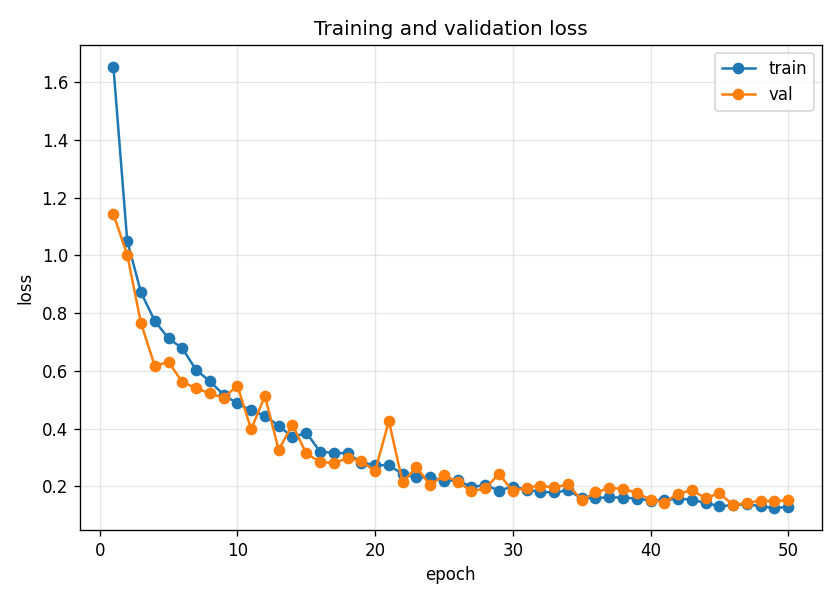
\includegraphics[width=0.78\textwidth]{../outputs/experiments/course_practical/runs/Final_multiclass/plots/loss_curve.png}
\caption{Loss curve of the final 10-class model.}
\label{fig:multiclass_loss}
\end{figure}

\begin{figure}[H]
\centering
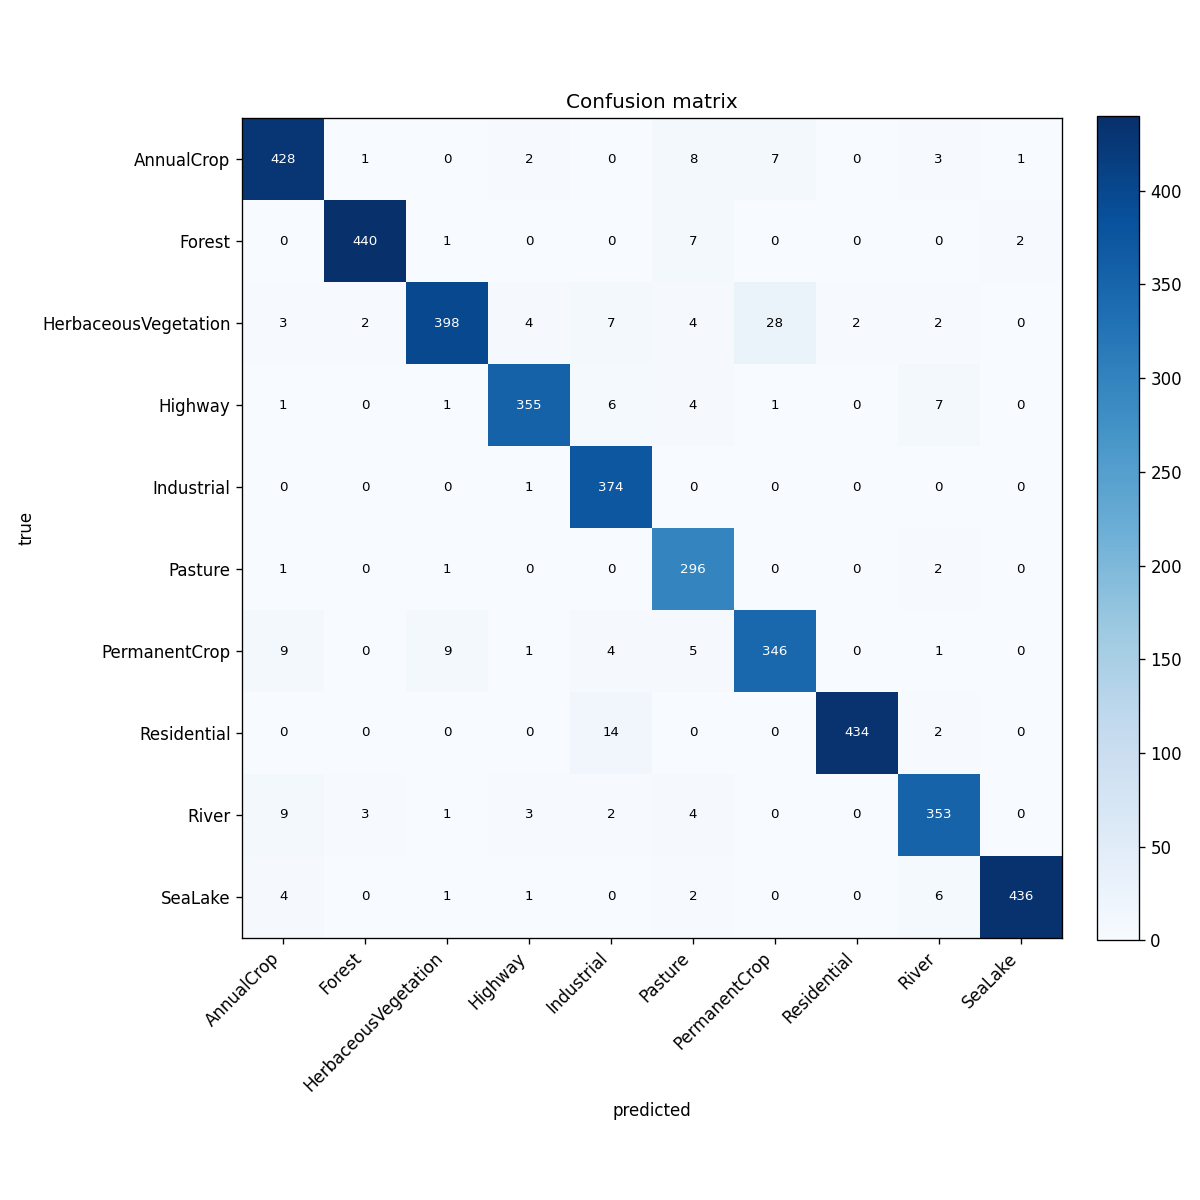
\includegraphics[width=0.78\textwidth]{../outputs/experiments/course_practical/runs/Final_multiclass/plots/confusion_matrix.png}
\caption{Confusion matrix of the final 10-class model on the test split.}
\label{fig:multiclass_cm}
\end{figure}

\begin{table}[H]
\centering
\caption{Per-class test results of the final 10-class model.}
\label{tab:per_class}
\small
\begin{tabular}{lrrrr}
\toprule
Class & Precision & Recall & F1 & Support \\
\midrule
AnnualCrop & 0.9407 & 0.9511 & 0.9459 & 450 \\
Forest & 0.9865 & 0.9778 & 0.9821 & 450 \\
HerbaceousVegetation & 0.9660 & 0.8844 & 0.9234 & 450 \\
Highway & 0.9673 & 0.9467 & 0.9569 & 375 \\
Industrial & 0.9189 & 0.9973 & 0.9565 & 375 \\
Pasture & 0.8970 & 0.9867 & 0.9397 & 300 \\
PermanentCrop & 0.9058 & 0.9227 & 0.9141 & 375 \\
Residential & 0.9954 & 0.9644 & 0.9797 & 450 \\
River & 0.9388 & 0.9413 & 0.9401 & 375 \\
SeaLake & 0.9932 & 0.9689 & 0.9809 & 450 \\
\bottomrule
\end{tabular}
\end{table}

The best F1 scores were achieved for Forest, SeaLake, and Residential. The
weakest scores were obtained for PermanentCrop, HerbaceousVegetation, and
Pasture. This is plausible because these classes can contain visually similar
vegetation patterns. The most frequent confusion in the test split was
HerbaceousVegetation predicted as PermanentCrop, with 28 images.

\subsubsection{Final Binary Classification}

For the binary task, the same selected configuration was used, but with two
output classes. The results are summarized in Table \ref{tab:final_binary}.

\begin{table}[H]
\centering
\caption{Final results for the binary classification task.}
\label{tab:final_binary}
\begin{tabular}{lrr}
\toprule
Metric & Validation & Test \\
\midrule
Loss & 0.0602 & 0.0660 \\
Accuracy & 0.9795 & 0.9795 \\
Macro-F1 & 0.9795 & 0.9795 \\
\bottomrule
\end{tabular}
\end{table}

On the test split, 3967 out of 4050 images were classified correctly. The
binary task is therefore clearly easier than the 10-class task. This is
expected because several similar vegetation classes no longer need to be
separated from each other.

\begin{figure}[H]
\centering
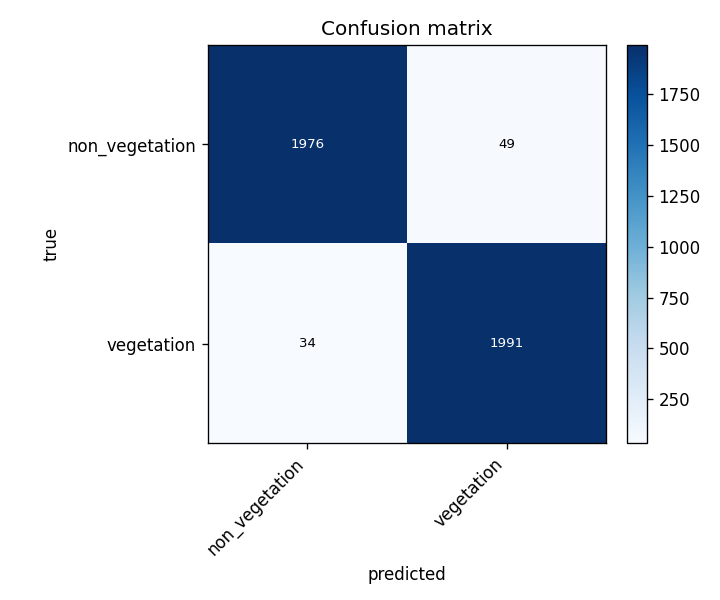
\includegraphics[width=0.7\textwidth]{../outputs/experiments/course_practical/runs/Final_binary/plots/confusion_matrix.png}
\caption{Confusion matrix of the final binary model on the test split.}
\label{fig:binary_cm}
\end{figure}

The binary confusion matrix shows 1976 correctly classified non-vegetation
images and 1991 correctly classified vegetation images. There were 49 cases
where non-vegetation was predicted as vegetation and 34 cases in the opposite
direction.

\section{Model 2: Transfer Learning with EfficientNet-B0}

\subsection{Methods}

Model 2 applies transfer learning and is evaluated with two pretrained backbones;
this section describes the first, EfficientNet-B0. In contrast to
the scratch CNN, this model is not initialized randomly. Instead, the
convolutional feature extractor is loaded with ImageNet-pretrained weights
\cite{tan2019efficientnet}. The original ImageNet classifier is replaced by a
new linear classification head with either ten outputs for the original
EuroSAT task or two outputs for the binary vegetation task.

EfficientNet-B0 was selected because it is a compact pretrained CNN and is
therefore suitable for a comparison with the smaller scratch model. Its main
advantage is that low-level and mid-level visual features such as edges,
textures, and object-like patterns are already represented in the pretrained
feature extractor. The model therefore does not need to learn all image
representations from the EuroSAT training split alone.

The input images are resized to $224 \times 224$ pixels, because this is the
standard input size of the ImageNet-pretrained EfficientNet-B0 model in
Torchvision. During training, horizontal flips, vertical flips, and rotations up
to 15 degrees are applied. Validation and test images are not randomly
augmented. All images are normalized with the standard ImageNet mean and
standard deviation, because the pretrained weights were trained with this
normalization scheme.

\begin{table}[H]
\centering
\caption{EfficientNet-B0 transfer learning setup.}
\label{tab:efficientnet_setup}
\small
\begin{tabularx}{\textwidth}{lX}
\toprule
Component & Configuration \\
\midrule
Base model & EfficientNet-B0 with ImageNet-pretrained weights \\
Input & RGB image resized to $3 \times 224 \times 224$ \\
Classifier & Replaced linear layer with 10 or 2 outputs \\
Loss function & \texttt{CrossEntropyLoss} \\
Optimizer & AdamW \\
Batch size & 64 \\
Epochs & 50 \\
Frozen phase & Epochs 1--5: train classifier head only \\
Fine-tuning phase & Epochs 6--50: unfreeze final two EfficientNet feature blocks \\
Model selection & Checkpoint with lowest validation loss \\
\bottomrule
\end{tabularx}
\end{table}

\subsection{Experimental Design}

The same stratified train/validation/test split as for Model 1 was used. This
keeps the comparison between the scratch CNN and the transfer learning model
fair. The two tasks are also identical: the 10-class EuroSAT classification and
the binary vegetation classification.

The training was performed in two stages. First, the EfficientNet feature
extractor was frozen and only the new classifier head was trained. This makes
the new output layer adapt to the EuroSAT labels without immediately changing
the pretrained feature representation. After five epochs, the final two feature
blocks of EfficientNet-B0 were unfrozen and fine-tuned with a smaller backbone
learning rate. This allows the model to adapt its higher-level features to the
satellite image domain.

The final hyperparameters were:

\begin{itemize}
  \item head learning rate: 0.001,
  \item backbone learning rate: 0.0001,
  \item weight decay: 0.0001,
  \item batch size: 64,
  \item seed: 42.
\end{itemize}

The test split was evaluated only after training, using the checkpoint with the
lowest validation loss.

\subsection{Results}

Table \ref{tab:efficientnet_results} summarizes the final EfficientNet-B0
results. For the 10-class task, the best checkpoint was selected after epoch 46.
For the binary task, the best checkpoint was selected after epoch 29.

\begin{table}[H]
\centering
\caption{Final results of the EfficientNet-B0 transfer learning model.}
\label{tab:efficientnet_results}
\small
\begin{tabular}{llrrr}
\toprule
Task & Split & Loss & Accuracy & Macro-F1 \\
\midrule
10-class & Validation & 0.0700 & 0.9793 & 0.9784 \\
10-class & Test & 0.0833 & 0.9726 & 0.9719 \\
Binary & Validation & 0.0130 & 0.9961 & 0.9961 \\
Binary & Test & 0.0184 & 0.9941 & 0.9941 \\
\bottomrule
\end{tabular}
\end{table}

Figure~\ref{fig:efficientnet_multiclass_curves} shows the loss and accuracy curves for the 10-class EfficientNet-B0 model. The strongest improvement occurs after switching from the frozen classifier-head phase to fine-tuning. The best checkpoint was selected in epoch 46 based on the lowest validation loss.

\begin{figure}[H]
    \centering
    \begin{minipage}{0.48\textwidth}
        \centering
        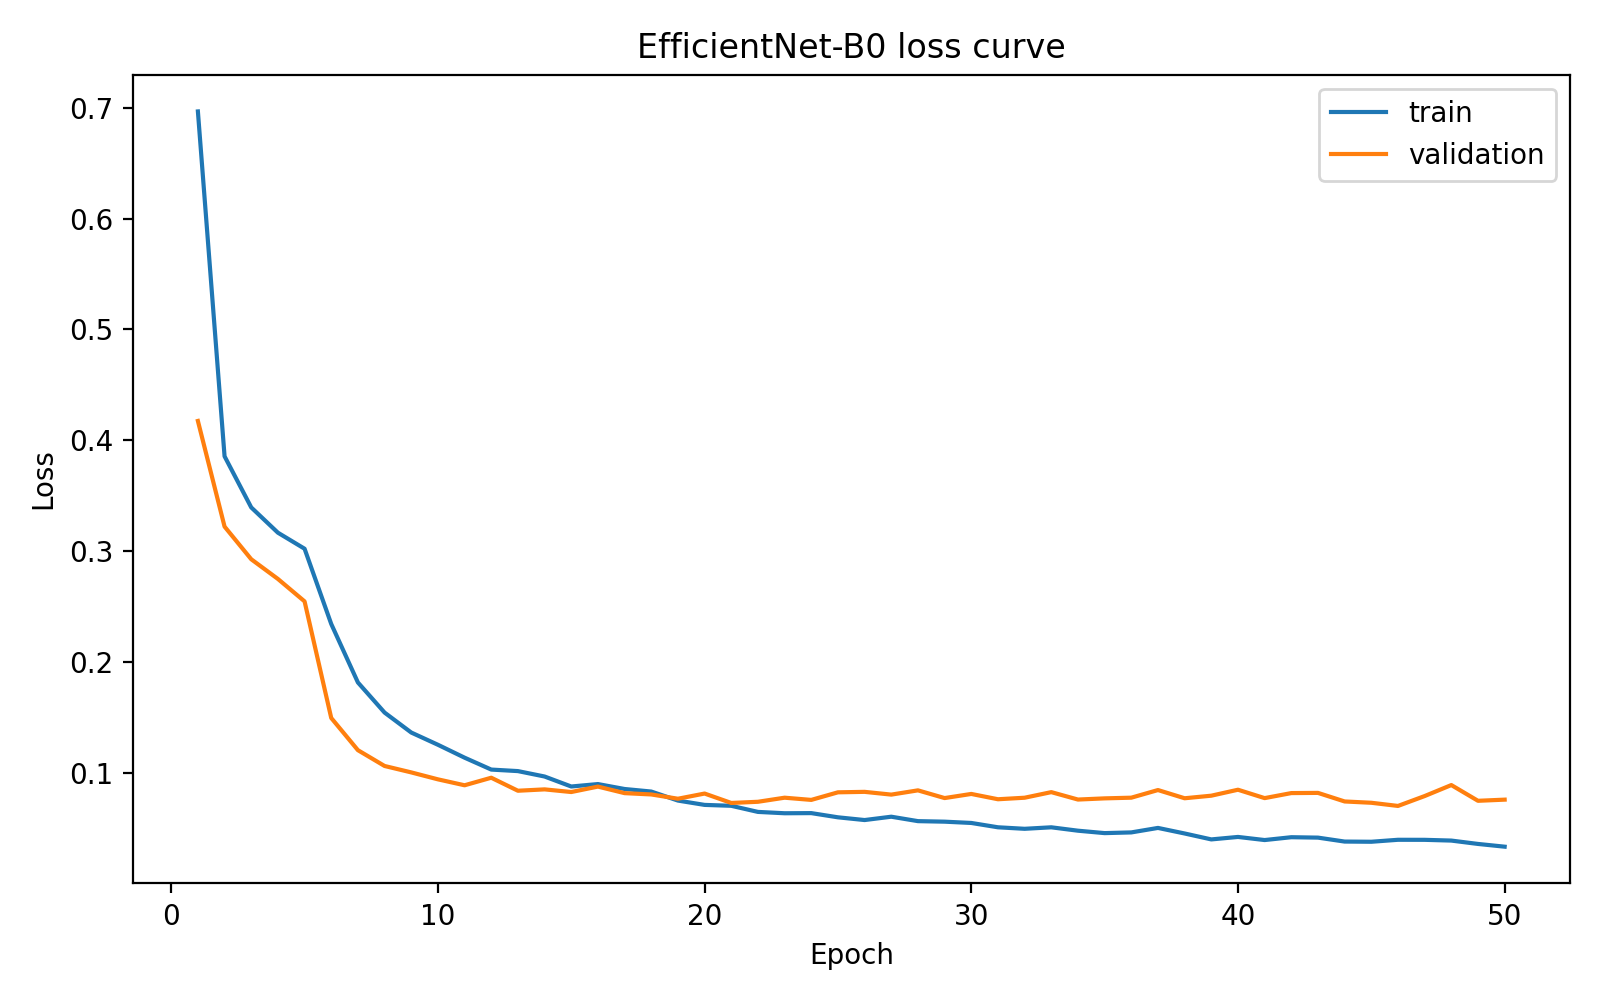
\includegraphics[width=\linewidth]{figures/efficientnet_b0/multiclass_loss_curve.png}
    \end{minipage}
    \hfill
    \begin{minipage}{0.48\textwidth}
        \centering
        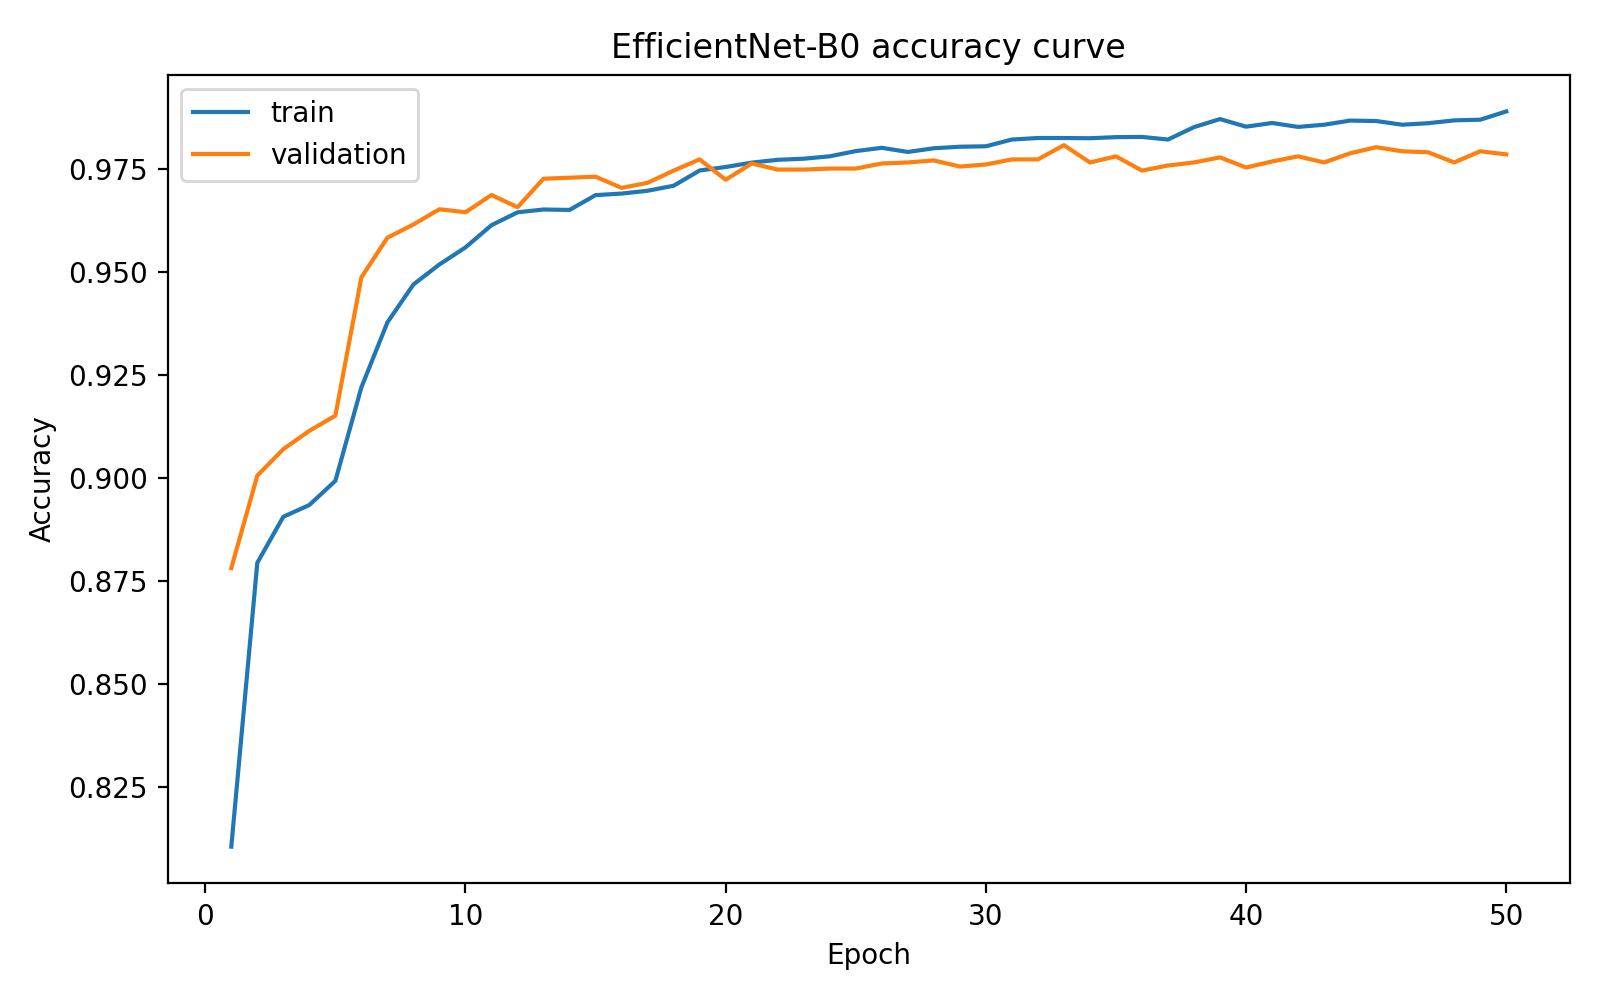
\includegraphics[width=\linewidth]{figures/efficientnet_b0/multiclass_accuracy_curve.png}
    \end{minipage}
    \caption{Loss and accuracy curves of the EfficientNet-B0 model on the 10-class task.}
    \label{fig:efficientnet_multiclass_curves}
\end{figure}

Figure~\ref{fig:efficientnet_multiclass_cm} shows the confusion matrix for the 10-class test split. The remaining errors mainly occur between visually similar land-use classes.

\begin{figure}[H]
    \centering
    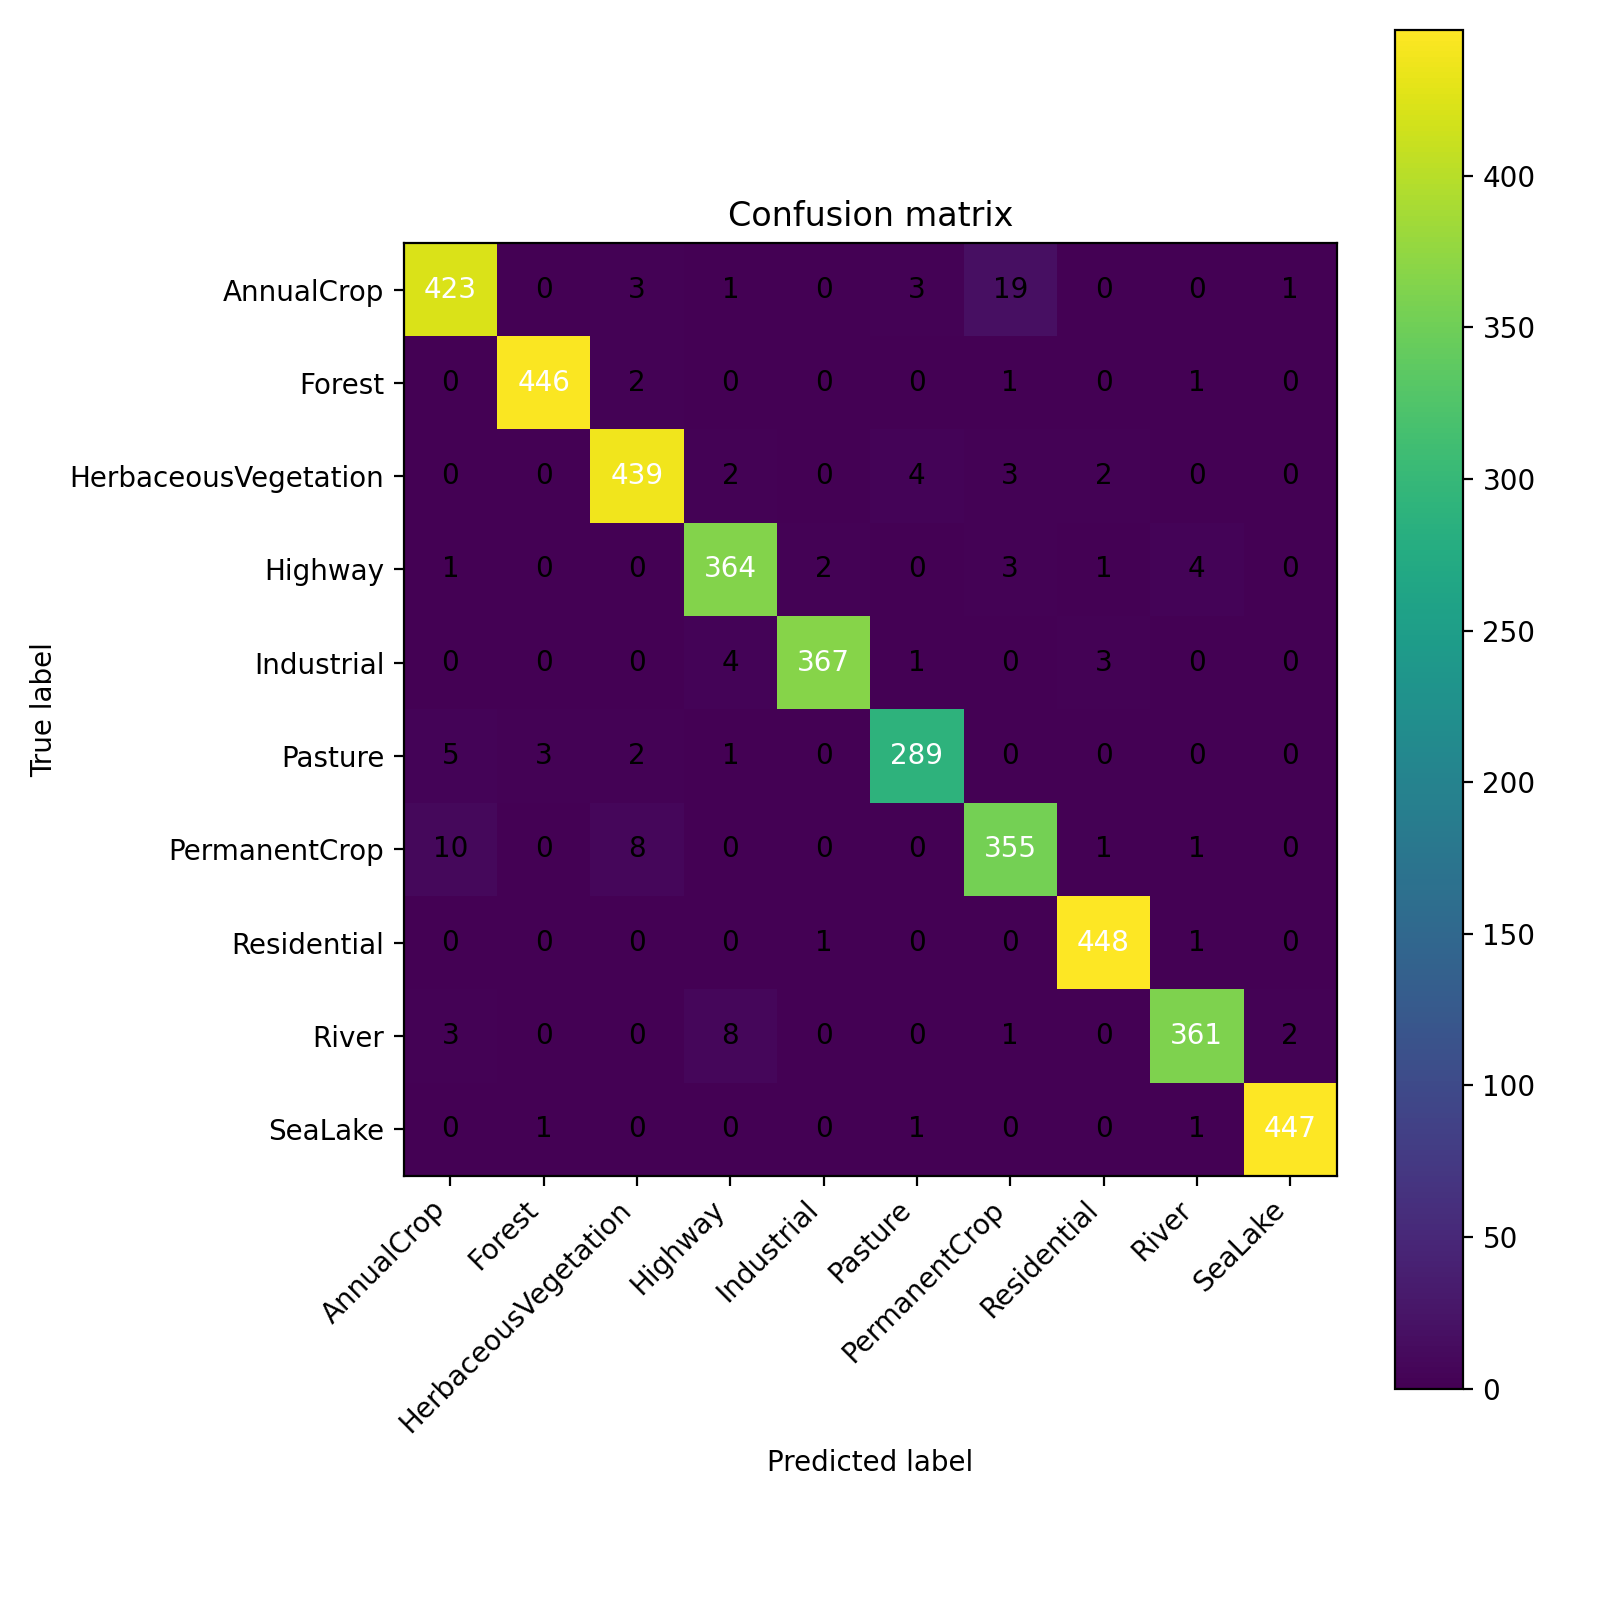
\includegraphics[width=0.70\textwidth]{figures/efficientnet_b0/multiclass_confusion_matrix.png}
    \caption{Confusion matrix of the EfficientNet-B0 model on the 10-class test split.}
    \label{fig:efficientnet_multiclass_cm}
\end{figure}

Figure~\ref{fig:efficientnet_binary_curves} shows the loss and accuracy curves for the binary vegetation classification task. The validation performance improves over the full training run, and the best checkpoint was selected in epoch 29.

\begin{figure}[H]
    \centering
    \begin{minipage}{0.48\textwidth}
        \centering
        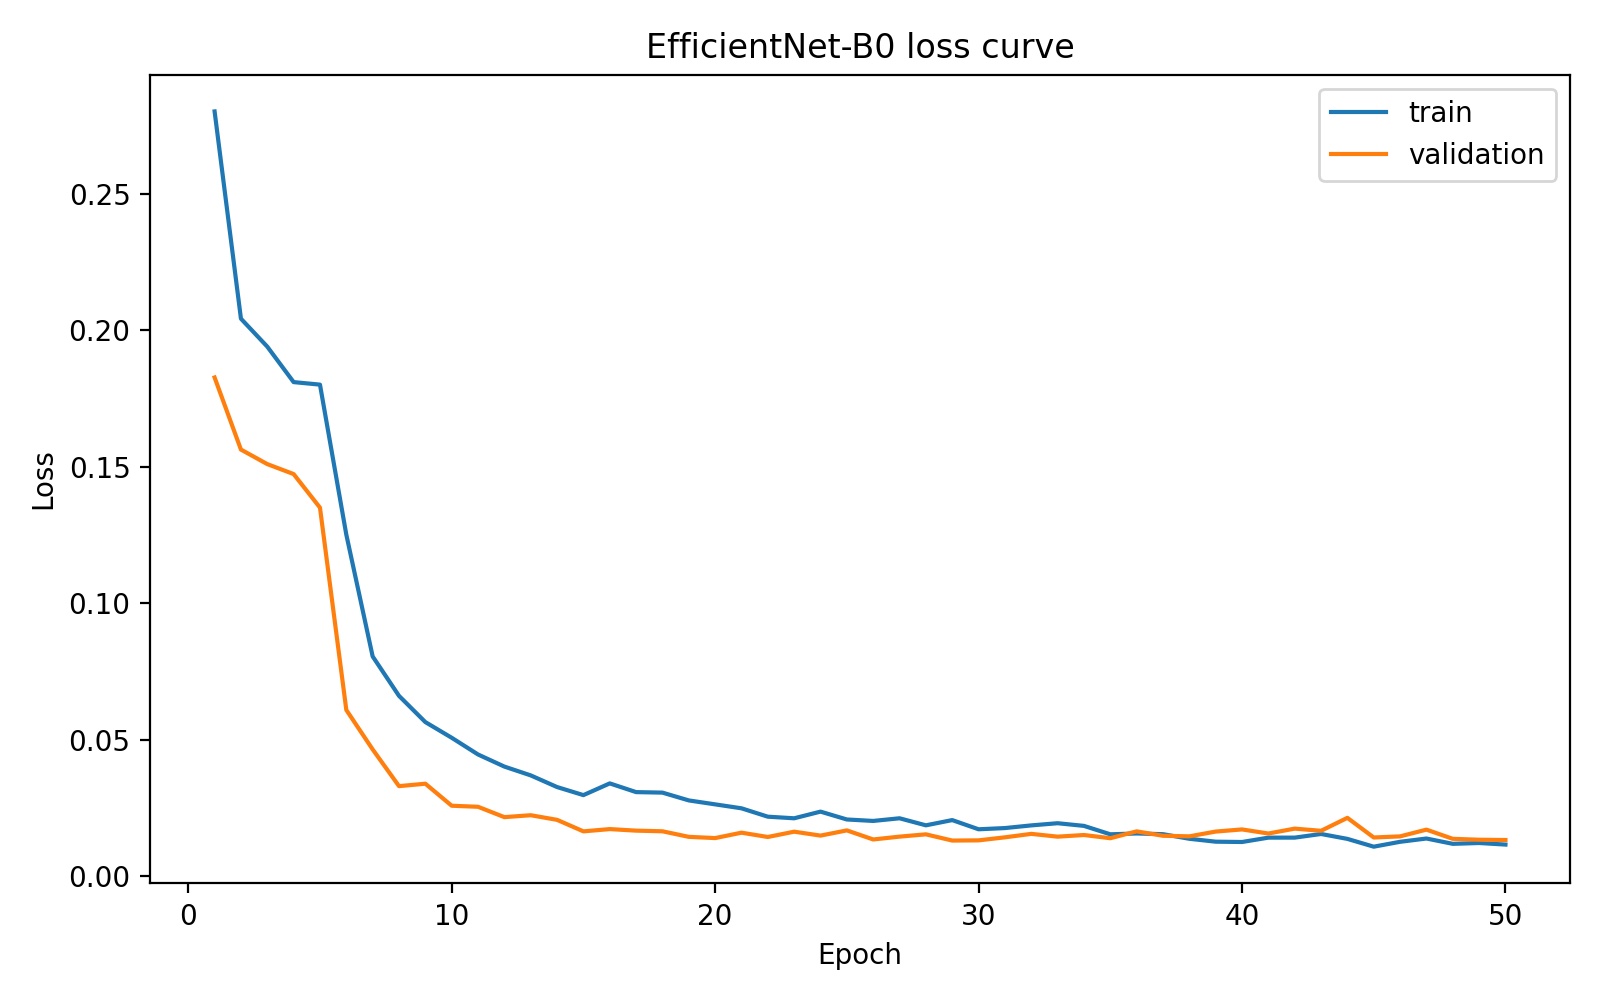
\includegraphics[width=\linewidth]{figures/efficientnet_b0/binary_loss_curve.png}
    \end{minipage}
    \hfill
    \begin{minipage}{0.48\textwidth}
        \centering
        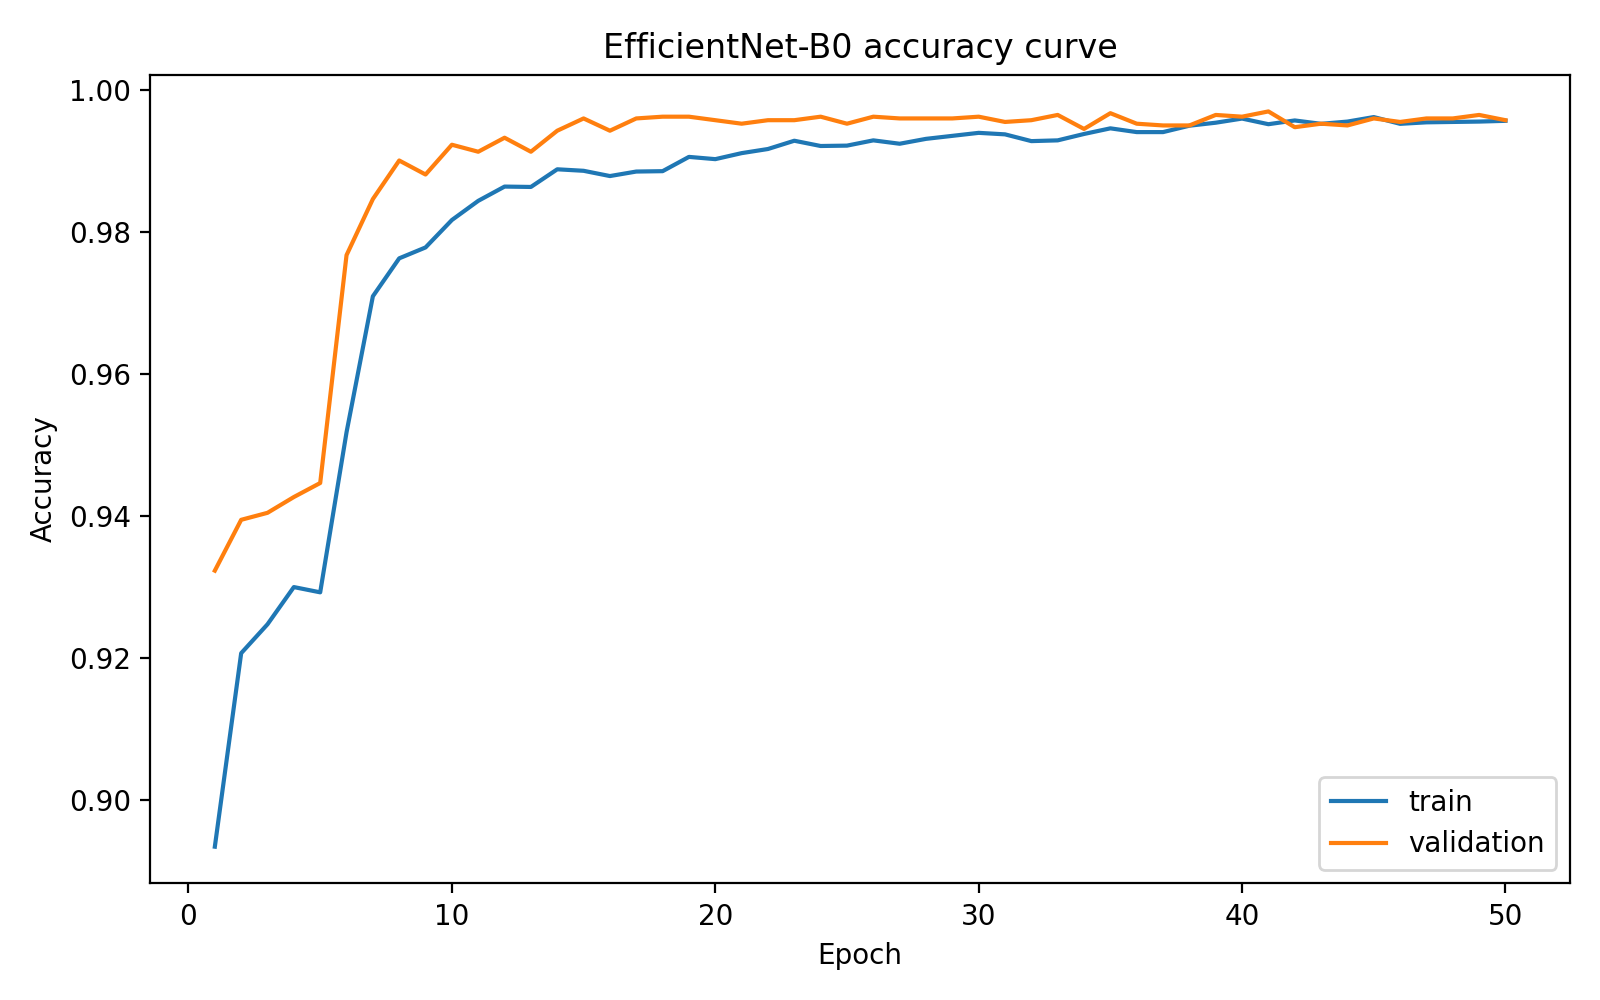
\includegraphics[width=\linewidth]{figures/efficientnet_b0/binary_accuracy_curve.png}
    \end{minipage}
    \caption{Loss and accuracy curves of the EfficientNet-B0 model on the binary task.}
    \label{fig:efficientnet_binary_curves}
\end{figure}

Figure~\ref{fig:efficientnet_binary_cm} shows the confusion matrix for the binary test split. The binary task produces fewer errors than the 10-class task because several visually similar vegetation classes are grouped into one shared class.

\begin{figure}[H]
    \centering
    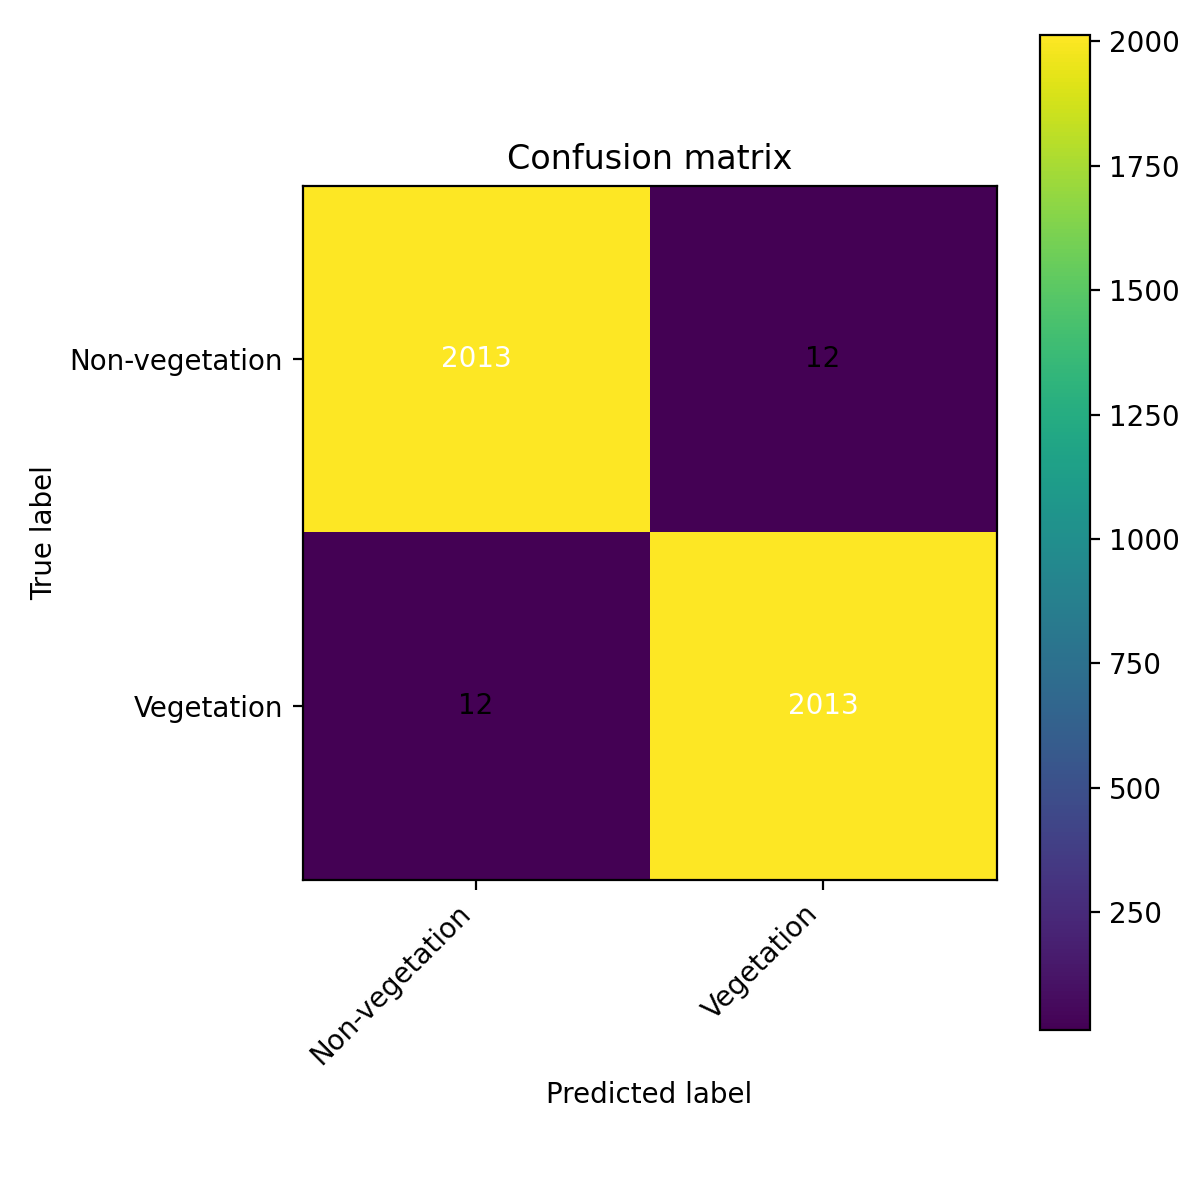
\includegraphics[width=0.60\textwidth]{figures/efficientnet_b0/binary_confusion_matrix.png}
    \caption{Confusion matrix of the EfficientNet-B0 model on the binary test split.}
    \label{fig:efficientnet_binary_cm}
\end{figure}

The 10-class model reached a test accuracy of 0.9726 and a test macro-F1 of
0.9719. This means that 3939 out of 4050 test images were classified correctly.
The epoch-46 checkpoint was used as the final model, based on the lowest
validation loss.

The binary task reached a test accuracy and macro-F1 of 0.9941. This means that
4026 out of 4050 test images were classified correctly. The binary task is
again easier than the full 10-class task, because visually similar vegetation
classes are grouped together.

\section{Model 2: Transfer Learning with ResNet-50}
\label{sec:model2}

\subsection{Methods}

The second backbone evaluated for Model 2 is a ResNet-50 pretrained on ImageNet
\cite{he2016resnet}. As with EfficientNet-B0, the network does not learn all
features from scratch but starts from weights that already encode general visual
features such as edges, textures, and shapes. These features can be reused for
satellite imagery classification with only minimal adaptation. Evaluating a
second, structurally different backbone makes the comparison with the scratch CNN
more robust: a consistent advantage across both ResNet-50 and EfficientNet-B0
indicates that the benefit stems from transfer learning itself rather than from a
single architecture.

ResNet-50 was chosen for this second backbone because it is a canonical, larger
deep-residual network and therefore complements the compact EfficientNet-B0: the
two cover different architecture families and capacities (roughly 25 versus 5
million parameters). It is a widely used reference for transfer learning, which
keeps the results comparable to the literature. Its clearly separated residual
stages (\texttt{layer1}--\texttt{layer4}) also make staged fine-tuning
straightforward, and high-quality ImageNet-pretrained weights
(\texttt{IMAGENET1K\_V2}) are readily available.

\subsubsection{ResNet-50 Architecture}

ResNet-50 is a deep residual network with 50 layers organized into four residual
stages, followed by a global average pooling layer and a fully connected
classification head. The defining feature of ResNet is the residual connection:
each block adds its input directly to its output before the activation. This
skip connection addresses the vanishing gradient problem and allows very deep
networks to be trained stably \cite{he2016resnet}.

\begin{table}[H]
\centering
\caption{ResNet-50 architecture overview. Feature map sizes assume 224$\times$224 input.}
\label{tab:resnet_architecture}
\begin{tabularx}{\textwidth}{lXX}
\toprule
Stage & Layers & Output size \\
\midrule
Input   & RGB image                          & 3$\times$224$\times$224 \\
Conv1   & 7$\times$7 conv, stride 2, MaxPool & 64$\times$56$\times$56  \\
Layer1  & 3 bottleneck blocks                & 256$\times$56$\times$56 \\
Layer2  & 4 bottleneck blocks                & 512$\times$28$\times$28 \\
Layer3  & 6 bottleneck blocks                & 1024$\times$14$\times$14 \\
Layer4  & 3 bottleneck blocks                & 2048$\times$7$\times$7  \\
Head    & GlobalAvgPool, Linear              & $C$ logits              \\
\bottomrule
\end{tabularx}
\end{table}

Each bottleneck block consists of three convolutional layers (1$\times$1, 3$\times$3,
1$\times$1) with batch normalization and ReLU activations. The 1$\times$1 layers
reduce and then restore the channel dimension, while the 3$\times$3 layer performs
the spatial feature extraction. This design keeps the parameter count manageable
despite the network depth.

\subsubsection{Transfer Learning Setup}

The pretrained weights were loaded from torchvision using the
\texttt{IMAGENET1K\_V2} checkpoint \cite{torchvision}. In the transfer learning
setup, the backbone is initially fully frozen and only the classification head is
replaced. The original fully connected layer, which outputs 1000 ImageNet
classes, is replaced by a new linear layer mapping the 2048-dimensional feature
vector to 10 outputs for the multiclass task or 2 outputs for the binary task.

All backbone parameters except those in the last residual stage (\texttt{layer4})
are kept frozen throughout training. The unfreezing of \texttt{layer4} allows the
network to adapt its highest-level features to the specific visual characteristics
of satellite imagery while keeping the low- and mid-level texture features fixed.
This strategy follows the standard practice of fine-tuning only the deeper layers,
since earlier layers in convolutional networks learn general low-level features
that transfer well across domains \cite{yosinski2014transferable}.

The key configuration differences from the scratch CNN are:

\begin{itemize}
  \item Input images are resized to 224$\times$224 (instead of 64$\times$64), matching the
    input resolution the backbone was pretrained on.
  \item Normalization uses ImageNet statistics: mean $[0.485, 0.456, 0.406]$ and
    standard deviation $[0.229, 0.224, 0.225]$ per channel. This ensures the
    input distribution matches what the frozen layers expect.
  \item The learning rate is set to $1\times10^{-4}$ (compared to $1\times10^{-3}$
    for the scratch CNN). A lower rate is important for fine-tuning to avoid
    overwriting the pretrained features with large gradient updates.
  \item The optimizer is Adam with weight decay $1\times10^{-4}$.
  \item Training runs for up to 50 epochs with early stopping after 8 epochs
    of no improvement in validation loss.
\end{itemize}

The number of trainable parameters with \texttt{layer4} unfrozen is 14{,}985{,}226.
For comparison, the fully frozen variant trains only the classification head,
giving 20{,}490 trainable parameters.

\subsection{Experimental Design}
\label{sec:model2_experiments}

Two sets of experiments were used to characterize the transfer learning model.

The first set tests \textbf{data efficiency}: how much labeled training data does
each model need to reach competitive accuracy? Both the ResNet and the scratch CNN
were trained on three progressively larger subsets of the training data, keeping
the full validation and test splits constant for fair comparison. Additionally, a
fully frozen ResNet was trained at full data as a baseline to isolate the
contribution of fine-tuning over using pretrained ImageNet features alone.

\begin{table}[H]
\centering
\caption{Data efficiency experiments. All runs use the multiclass task and
evaluate on the full test split ($n=4050$).}
\label{tab:data_efficiency_exp}
\begin{tabular}{llrrr}
\toprule
ID & Model & Train images & Test Acc. & Test Macro-F1 \\
\midrule
S-50    & Scratch CNN       &    500 & 0.7017 & 0.6904 \\
S-200   & Scratch CNN       &  2{,}000 & 0.8430 & 0.8379 \\
S-full  & Scratch CNN       & 18{,}899 & 0.9479 & 0.9462 \\
\midrule
R-50    & ResNet (layer4)   &    500 & 0.9284 & 0.9263 \\
R-200   & ResNet (layer4)   &  2{,}000 & 0.9556 & 0.9542 \\
R-full  & ResNet (layer4)   & 18{,}899 & 0.9817 & 0.9812 \\
\midrule
R-frz   & ResNet (frozen)   & 18{,}899 & 0.9373 & 0.9347 \\
\bottomrule
\end{tabular}
\end{table}

The second set applies the same data efficiency design to the \textbf{binary
vegetation task}.

\begin{table}[H]
\centering
\caption{Data efficiency experiments on the binary classification task.
Test split $n=4050$.}
\label{tab:data_efficiency_binary}
\begin{tabular}{llrrr}
\toprule
ID & Model & Train images & Test Acc. & Test Macro-F1 \\
\midrule
S-50-b   & Scratch CNN     &    500 & 0.8691 & 0.8691 \\
S-200-b  & Scratch CNN     &  2{,}000 & 0.9081 & 0.9081 \\
S-full-b & Scratch CNN     & 18{,}899 & 0.9741 & 0.9741 \\
\midrule
R-50-b   & ResNet (layer4) &    500 & 0.9753 & 0.9753 \\
R-200-b  & ResNet (layer4) &  2{,}000 & 0.9889 & 0.9889 \\
R-full-b & ResNet (layer4) & 18{,}899 & 0.9938 & 0.9938 \\
\bottomrule
\end{tabular}
\end{table}

\subsection{Results}

\subsubsection{Final 10-Class Classification}

The final ResNet model (R-full, \texttt{layer4} unfrozen, full training data)
achieves the results shown in Table \ref{tab:resnet_final_multiclass}. The model
converged in 15 epochs before early stopping triggered.

\begin{table}[H]
\centering
\caption{Final ResNet-50 results for the 10-class classification task.}
\label{tab:resnet_final_multiclass}
\begin{tabular}{lrr}
\toprule
Metric & Validation & Test \\
\midrule
Loss     & 0.0732 & 0.0618 \\
Accuracy & 0.9780 & 0.9817 \\
Macro-F1 & 0.9770 & 0.9812 \\
\bottomrule
\end{tabular}
\end{table}

\begin{figure}[H]
\centering
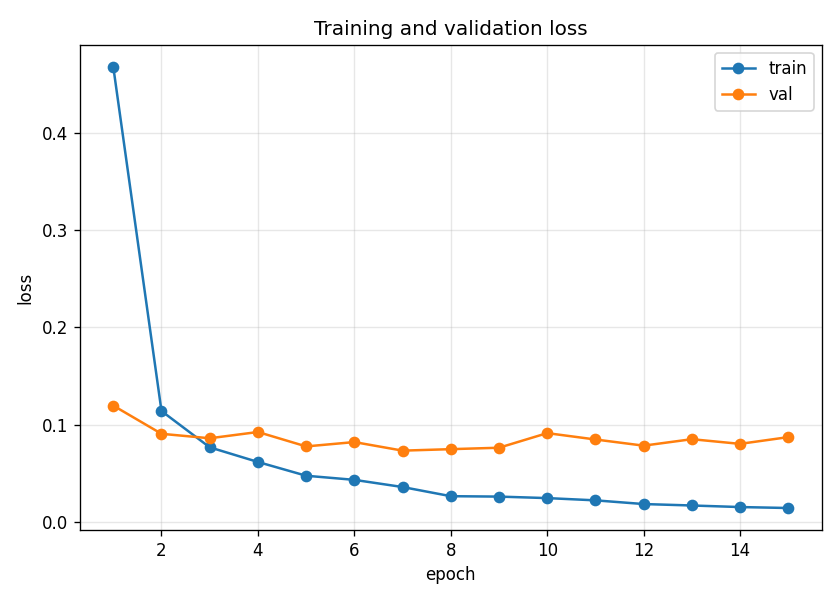
\includegraphics[width=0.78\textwidth]{../outputs/experiments/scratch_vs_transfer/runs/resnet_full/plots/loss_curve.png}
\caption{Loss curve of the final ResNet-50 10-class model.}
\label{fig:resnet_loss}
\end{figure}

\begin{figure}[H]
\centering
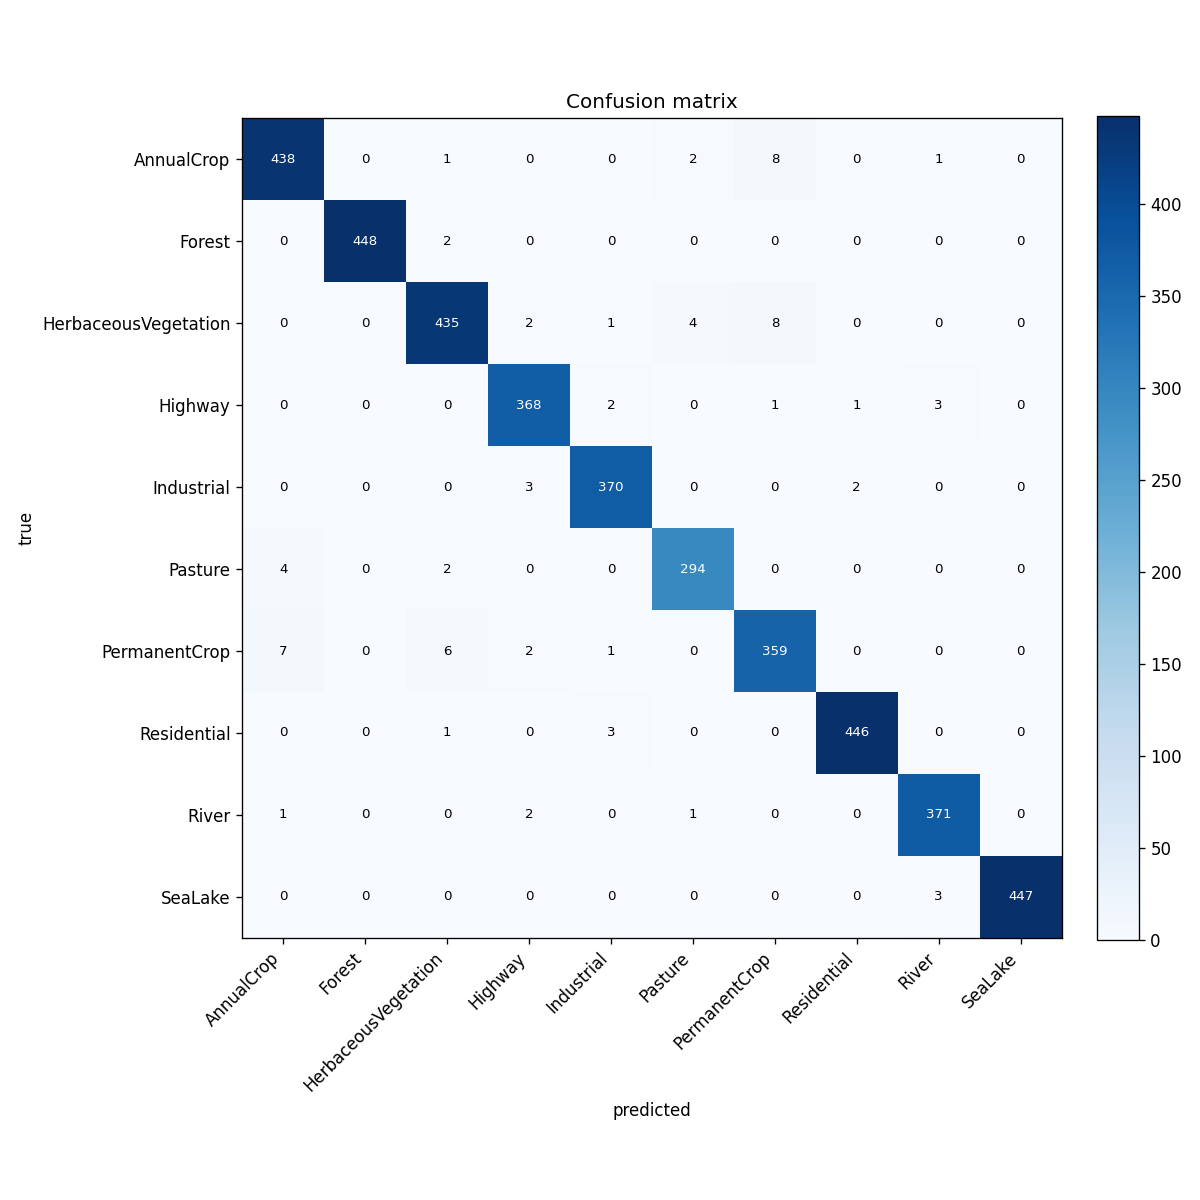
\includegraphics[width=0.78\textwidth]{../outputs/experiments/scratch_vs_transfer/runs/resnet_full/plots/confusion_matrix.png}
\caption{Confusion matrix of the final ResNet-50 10-class model on the test split.}
\label{fig:resnet_cm}
\end{figure}

\begin{table}[H]
\centering
\caption{Per-class test results of the final ResNet-50 10-class model.}
\label{tab:resnet_per_class}
\small
\begin{tabular}{lrrrr}
\toprule
Class & Precision & Recall & F1 & Support \\
\midrule
AnnualCrop            & 0.9733 & 0.9733 & 0.9733 & 450 \\
Forest                & 1.0000 & 0.9956 & 0.9978 & 450 \\
HerbaceousVegetation  & 0.9732 & 0.9667 & 0.9699 & 450 \\
Highway               & 0.9761 & 0.9813 & 0.9787 & 375 \\
Industrial            & 0.9814 & 0.9867 & 0.9840 & 375 \\
Pasture               & 0.9767 & 0.9800 & 0.9784 & 300 \\
PermanentCrop         & 0.9548 & 0.9573 & 0.9561 & 375 \\
Residential           & 0.9933 & 0.9911 & 0.9922 & 450 \\
River                 & 0.9815 & 0.9893 & 0.9854 & 375 \\
SeaLake               & 1.0000 & 0.9933 & 0.9967 & 450 \\
\bottomrule
\end{tabular}
\end{table}

On the test split, 3976 out of 4050 images were classified correctly, leaving
74 misclassifications. The weakest class is PermanentCrop (F1 0.9561), which is
also the hardest class for the scratch CNN. The strongest classes are Forest and
SeaLake, both achieving near-perfect precision. The overall per-class scores are
notably more uniform than for the scratch CNN, suggesting that the pretrained
features generalize better across visually similar classes.

\subsubsection{Final Binary Classification}

The binary ResNet model (R-full-b) achieves the results shown in Table
\ref{tab:resnet_final_binary}. The model converged in 12 epochs.

\begin{table}[H]
\centering
\caption{Final ResNet-50 results for the binary classification task.}
\label{tab:resnet_final_binary}
\begin{tabular}{lrr}
\toprule
Metric & Validation & Test \\
\midrule
Loss     & 0.0165 & --- \\
Accuracy & 0.9943 & 0.9938 \\
Macro-F1 & 0.9943 & 0.9938 \\
\bottomrule
\end{tabular}
\end{table}

\begin{figure}[H]
\centering
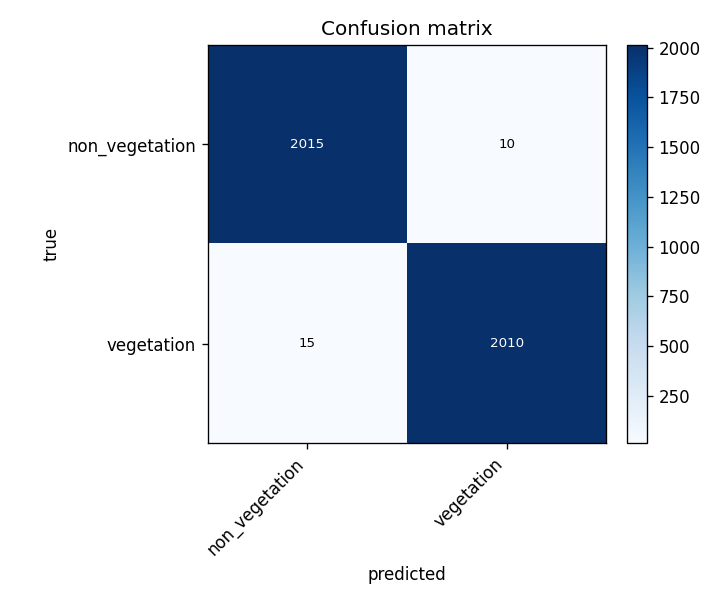
\includegraphics[width=0.7\textwidth]{../outputs/experiments/scratch_vs_transfer/runs/resnet_full_binary/plots/confusion_matrix.png}
\caption{Confusion matrix of the final ResNet-50 binary model on the test split.}
\label{fig:resnet_binary_cm}
\end{figure}

On the binary task the model misclassifies only 25 out of 4050 images. Both
vegetation and non-vegetation classes are handled with nearly equal accuracy,
indicating that the pretrained features already capture the spectral and textural
distinction between these two categories very reliably.

\section{Discussion and Limitations}

\subsection{Model 1 Interpretation}

The experiments show that a relatively small scratch CNN can already achieve
strong results on EuroSAT RGB. The architecture alone was not the only important
part. The training configuration also mattered. The best validation result was
obtained only after combining augmentation, dropout, weight decay, and SGD with
momentum.

The binary classification task
reached a test macro-F1 of 0.9795, while the 10-class classification reached
0.9519. This is expected because the binary task groups several similar classes
together. Vegetation classes such as Pasture, PermanentCrop,
HerbaceousVegetation, and AnnualCrop can be difficult to separate in RGB images.

One advantage of the chosen procedure is the clean separation between training,
validation, and test data. Normalization was computed only from the training
data, and the test split was not used for hyperparameter selection. Therefore,
the final test scores are more meaningful than they would be if the test split
had been used repeatedly during model tuning.

\subsection{ResNet Transfer Learning Interpretation}

The ResNet-50 transfer learning model achieves a test macro-F1 of 0.9812 on the
10-class task, compared to 0.9519 for the scratch CNN. The improvement is
moderate in absolute terms, but the data efficiency experiments reveal a much
larger story.

The frozen ResNet baseline, which trains only the linear classification head
(20{,}490 parameters) while keeping all backbone weights fixed, reaches a test
accuracy of 93.7\%. This means that ImageNet features alone, without any
fine-tuning, already outperform the fully trained scratch CNN at 500 and 2{,}000
training images. It confirms that the backbone has learned feature representations
that transfer directly to satellite land-use classification.

Fine-tuning \texttt{layer4} on top of the frozen features adds a further 4.4
percentage points at full data, pushing test accuracy from 93.7\% to 98.2\%.
This marginal cost (adapting roughly 14.7 million parameters instead of 20{,}490)
is justified by the consistent gain across all data sizes.

One limitation of the transfer learning approach is the increased computational
cost per epoch. With 224$\times$224 inputs and a 50-layer backbone, each epoch
takes approximately 151 seconds on Apple Silicon MPS, compared to 8 seconds for
the scratch CNN. However, the ResNet requires far fewer epochs to converge
(15 vs.\ 42 for the scratch CNN at full data), so the total wall-clock training
time is roughly 37 minutes versus 6 minutes. For applications where training
time matters more than final accuracy, the scratch CNN remains a practical choice.

\subsection{Model Comparison}

Table \ref{tab:model_comparison} compares the scratch CNN with the two Model 2
transfer-learning backbones across both tasks. Both pretrained backbones
outperform the scratch CNN on both tasks: ResNet-50 achieves the best 10-class
result, while EfficientNet-B0 is marginally the best on the binary task.

\begin{table}[H]
\centering
\caption{Final model comparison on the full test split ($n=4050$).}
\label{tab:model_comparison}
\small
\begin{tabular}{llrrrr}
\toprule
Model & Task & Val Acc. & Val F1 & Test Acc. & Test F1 \\
\midrule
Scratch CNN        & 10-class & 0.9573 & 0.9557 & 0.9531 & 0.9519 \\
Scratch CNN        & Binary   & 0.9795 & 0.9795 & 0.9795 & 0.9795 \\
EfficientNet-B0    & 10-class & 0.9793 & 0.9784 & 0.9726 & 0.9719 \\
EfficientNet-B0    & Binary   & 0.9961 & 0.9961 & 0.9941 & 0.9941 \\
ResNet-50 (layer4) & 10-class & 0.9780 & 0.9770 & 0.9817 & 0.9812 \\
ResNet-50 (layer4) & Binary   & 0.9943 & 0.9943 & 0.9938 & 0.9938 \\
\bottomrule
\end{tabular}
\end{table}

For the 10-class task, both pretrained backbones outperformed the scratch CNN on
the test set. EfficientNet-B0 reached a test macro-F1 of 0.9719 and ResNet-50
reached 0.9812, compared with 0.9519 for the scratch CNN. ResNet-50, fine-tuned
through \texttt{layer4}, achieved the best 10-class result overall: it improved
test accuracy by 2.9 percentage points over the scratch CNN (0.9817 vs.\ 0.9531),
with EfficientNet-B0 following closely. This confirms that the pretrained features
transfer well to EuroSAT once the backbones are fine-tuned for enough epochs.

For the binary task, both pretrained models performed better than the scratch
CNN. EfficientNet-B0 reached a test macro-F1 of 0.9941 and ResNet-50 reached
0.9938, compared with 0.9795 for the scratch CNN. The two backbones are
essentially tied on this task, with EfficientNet-B0 marginally ahead. This
suggests that pretrained visual features are especially useful when the target
decision boundary is less fine-grained. Separating vegetation from non-vegetation does not require
distinguishing all visually similar crop and vegetation subclasses.

The data efficiency comparison in Tables \ref{tab:data_efficiency_exp} and
\ref{tab:data_efficiency_binary} is more informative than the full-data numbers
alone. At 500 training images, the ResNet (layer4) achieves a test accuracy of
92.8\% on the 10-class task, while the scratch CNN reaches only 70.2\%. This
22.6 percentage point gap shrinks to 3.4 points at full data. The result shows
that transfer learning is most beneficial in low-data regimes, where the
pretrained features compensate for the lack of labeled examples. When sufficient
data is available, a well-regularized scratch CNN narrows the gap substantially.

The binary data efficiency results are even more striking. At 500 images, the
ResNet already achieves 97.5\% test accuracy, while the scratch CNN reaches
86.9\%. The scratch CNN only surpasses 97\% when trained on the full dataset.
Transfer learning therefore reaches the scratch CNN's full-data performance using
roughly 2.6\% of the training data.

\begin{table}[H]
\centering
\caption{Summary of key comparison metrics between the scratch CNN and ResNet-50.}
\label{tab:comparison_summary}
\small
\begin{tabular}{lrr}
\toprule
Metric & Scratch CNN & ResNet-50 (layer4) \\
\midrule
Trainable parameters          & 390{,}986   & 14{,}985{,}226 \\
Input resolution              & 64$\times$64    & 224$\times$224     \\
Epochs to converge (full data)& 42          & 15                 \\
Time per epoch (full data)    & $\sim$8\,s  & $\sim$151\,s       \\
Total training time           & $\sim$6\,min & $\sim$38\,min     \\
10-class test accuracy        & 0.9531      & 0.9817             \\
10-class test macro-F1        & 0.9519      & 0.9812             \\
Binary test accuracy          & 0.9795      & 0.9938             \\
Test acc.\ at 500 train images (10-class) & 0.7017 & 0.9284      \\
\bottomrule
\end{tabular}
\end{table}

Overall, both approaches are valid. The scratch CNN is easiest to understand
and directly demonstrates the training process from the course. For Model 2,
both transfer-learning backbones use external pretraining knowledge and a larger
input resolution: EfficientNet-B0 is a strong, parameter-efficient baseline that
matches ResNet-50 on the binary task, while ResNet-50 gives the best 10-class
accuracy and by far the best data efficiency, at the cost of higher per-epoch
compute. The fact that both pretrained backbones outperform the scratch CNN on
both tasks indicates that the benefit comes from transfer learning itself rather
than from a single architecture.

\subsection{Limitations}

There are several limitations. First, only RGB information was used. Sentinel-2
data contains additional spectral bands that could be useful for distinguishing
vegetation, water, and built-up areas. Both pretrained backbones expect
three-channel input, so these additional bands were not used in the transfer
learning models.

Second, all models were evaluated with one fixed seed. Multiple training runs
with different seeds would give a better estimate of variance.

\section{Conclusion}

In this project, EuroSAT RGB is used for two related classification tasks. The
first completed model is a CNN implemented and trained from scratch. Its final
configuration was not chosen arbitrarily, but selected from several validation
experiments. SGD with momentum, combined with augmentation, dropout, and weight
decay, gave the best validation results for the scratch CNN.

The final scratch CNN achieved a test accuracy of 0.9531 and a macro-F1 of
0.9519 on the 10-class task. On the binary task, it achieved 0.9795 accuracy and
0.9795 macro-F1. The results show that a compact, self-trained CNN works well on
EuroSAT RGB. The remaining errors mainly occur between visually similar classes,
especially within the vegetation categories.

Model 2 is a transfer learning approach, evaluated with two ImageNet-pretrained
backbones. The first, EfficientNet-B0, had its classifier replaced for the
EuroSAT tasks and was trained in two phases: first with a frozen feature
extractor and then with the final EfficientNet blocks unfrozen.

The second backbone for Model 2, ResNet-50, was evaluated to test whether the
transfer-learning advantage holds across architectures. It achieved a test
accuracy of 0.9817 and a macro-F1 of 0.9812 on the
10-class task, and 0.9938 on the binary task. The data efficiency experiments
show that the pretrained model reaches competitive accuracy with far less
labeled data: at only 500 training images it achieves 92.8\% test accuracy on
the 10-class task, compared to 70.2\% for the scratch CNN. The gap narrows when
the full dataset is available, but the ResNet consistently outperforms the
scratch CNN across all data sizes and both tasks.

The results show that both approaches work well on EuroSAT. Both Model 2 backbones
outperformed the scratch CNN on both tasks. ResNet-50 achieved the best 10-class
result (macro-F1 0.9812), while EfficientNet-B0 was marginally best on the binary
task (macro-F1 0.9941, versus 0.9938 for ResNet-50). The binary task was easier
for all models because
several visually similar
vegetation classes were merged into one class. The remaining errors mainly occur
between visually similar land use categories.

A useful extension would be to use all Sentinel-2 spectral bands instead of RGB
only. This would require either adapting the first layer of a pretrained model
or using a model designed for multispectral satellite images.

\printbibliography

\end{document}
